\documentclass{extbook}[14pt]
\usepackage{multicol, enumerate, enumitem, hyperref, color, soul, setspace, parskip, fancyhdr, amssymb, amsthm, amsmath, latexsym, units, mathtools}
\everymath{\displaystyle}
\usepackage[headsep=0.5cm,headheight=0cm, left=1 in,right= 1 in,top= 1 in,bottom= 1 in]{geometry}
\usepackage{dashrule}  % Package to use the command below to create lines between items
\newcommand{\litem}[1]{\item #1

\rule{\textwidth}{0.4pt}}
\pagestyle{fancy}
\lhead{}
\chead{Answer Key for Progress Quiz 3 Version ALL}
\rhead{}
\lfoot{3012-8528}
\cfoot{}
\rfoot{Summer C 2021}
\begin{document}
\textbf{This key should allow you to understand why you choose the option you did (beyond just getting a question right or wrong). \href{https://xronos.clas.ufl.edu/mac1105spring2020/courseDescriptionAndMisc/Exams/LearningFromResults}{More instructions on how to use this key can be found here}.}

\textbf{If you have a suggestion to make the keys better, \href{https://forms.gle/CZkbZmPbC9XALEE88}{please fill out the short survey here}.}

\textit{Note: This key is auto-generated and may contain issues and/or errors. The keys are reviewed after each exam to ensure grading is done accurately. If there are issues (like duplicate options), they are noted in the offline gradebook. The keys are a work-in-progress to give students as many resources to improve as possible.}

\rule{\textwidth}{0.4pt}

\begin{enumerate}\litem{
Describe the end behavior of the polynomial below.
\[ f(x) = -3(x + 5)^{4}(x - 5)^{7}(x - 7)^{4}(x + 7)^{6} \]The solution is the graph below, which is option A.
    \begin{center}
        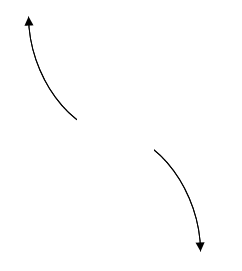
\includegraphics[width=0.3\textwidth]{../Figures/polyEndBehaviorCopyAA.png}
    \end{center}\begin{enumerate}[label=\Alph*.]
\begin{multicols}{2}
\item 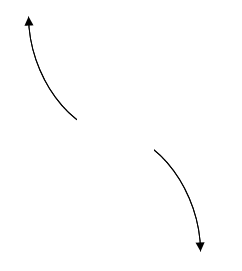
\includegraphics[width = 0.3\textwidth]{../Figures/polyEndBehaviorCopyAA.png}
\item 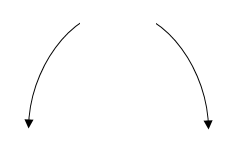
\includegraphics[width = 0.3\textwidth]{../Figures/polyEndBehaviorCopyBA.png}
\item 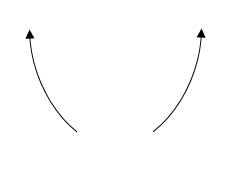
\includegraphics[width = 0.3\textwidth]{../Figures/polyEndBehaviorCopyCA.png}
\item 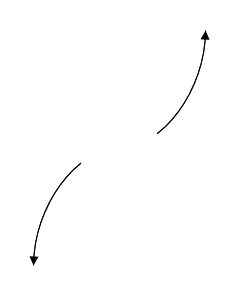
\includegraphics[width = 0.3\textwidth]{../Figures/polyEndBehaviorCopyDA.png}
\end{multicols}\item None of the above.\end{enumerate}
\textbf{General Comment:} Remember that end behavior is determined by the leading coefficient AND whether the \textbf{sum} of the multiplicities is positive or negative.
}
\litem{
Describe the zero behavior of the zero $x = 3$ of the polynomial below.
\[ f(x) = 6(x - 3)^{8}(x + 3)^{13}(x - 4)^{9}(x + 4)^{12} \]The solution is the graph below, which is option B.
    \begin{center}
        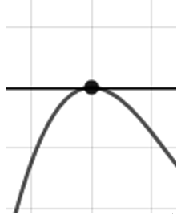
\includegraphics[width=0.3\textwidth]{../Figures/polyZeroBehaviorBA.png}
    \end{center}\begin{enumerate}[label=\Alph*.]
\begin{multicols}{2}
\item 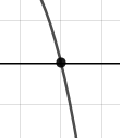
\includegraphics[width = 0.3\textwidth]{../Figures/polyZeroBehaviorAA.png}
\item 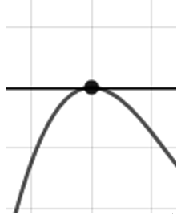
\includegraphics[width = 0.3\textwidth]{../Figures/polyZeroBehaviorBA.png}
\item 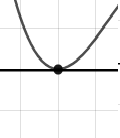
\includegraphics[width = 0.3\textwidth]{../Figures/polyZeroBehaviorCA.png}
\item 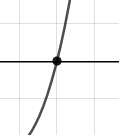
\includegraphics[width = 0.3\textwidth]{../Figures/polyZeroBehaviorDA.png}
\end{multicols}\item None of the above.\end{enumerate}
\textbf{General Comment:} You will need to sketch the entire graph, then zoom in on the zero the question asks about.
}
\litem{
Which of the following equations \textit{could} be of the graph presented below?

\begin{center}
    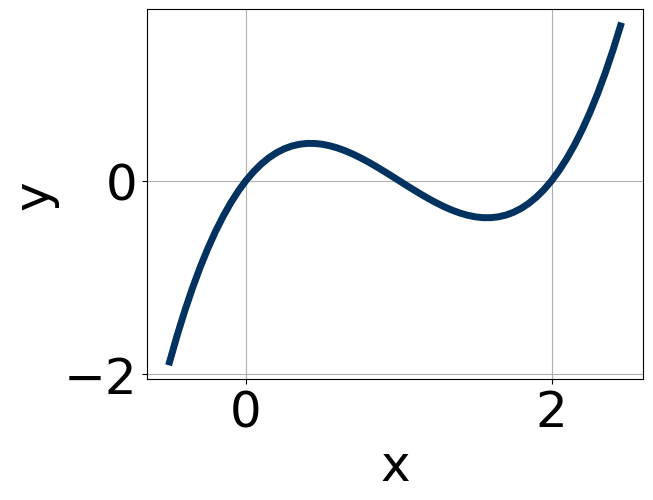
\includegraphics[width=0.5\textwidth]{../Figures/polyGraphToFunctionA.png}
\end{center}


The solution is \( 18x^{7} (x - 2)^{7} (x - 1)^{5} \), which is option C.\begin{enumerate}[label=\Alph*.]
\item \( 4x^{7} (x - 2)^{10} (x - 1)^{5} \)

The factor $2$ should have been an odd power.
\item \( -8x^{9} (x - 2)^{6} (x - 1)^{5} \)

The factor $(x - 2)$ should have an odd power and the leading coefficient should be the opposite sign.
\item \( 18x^{7} (x - 2)^{7} (x - 1)^{5} \)

* This is the correct option.
\item \( 7x^{10} (x - 2)^{8} (x - 1)^{11} \)

The factors $2$ and $0$ have have been odd power.
\item \( -12x^{9} (x - 2)^{5} (x - 1)^{5} \)

This corresponds to the leading coefficient being the opposite value than it should be.
\end{enumerate}

\textbf{General Comment:} General Comments: Draw the x-axis to determine which zeros are touching (and so have even multiplicity) or cross (and have odd multiplicity).
}
\litem{
Construct the lowest-degree polynomial given the zeros below. Then, choose the intervals that contain the coefficients of the polynomial in the form $x^3+bx^2+cx+d$.
\[ 4 + 5 i \text{ and } 2 \]The solution is \( x^{3} -10 x^{2} +57 x -82 \), which is option D.\begin{enumerate}[label=\Alph*.]
\item \( b \in [7, 16], c \in [56, 57.3], \text{ and } d \in [81, 86.3] \)

$x^{3} +10 x^{2} +57 x + 82$, which corresponds to multiplying out $(x-(4 + 5 i))(x-(4 - 5 i))(x + 2)$.
\item \( b \in [0, 2], c \in [-6.8, -1.8], \text{ and } d \in [3.8, 8.5] \)

$x^{3} + x^{2} -6 x + 8$, which corresponds to multiplying out $(x -4)(x -2)$.
\item \( b \in [0, 2], c \in [-8.8, -6.5], \text{ and } d \in [8.4, 13.1] \)

$x^{3} + x^{2} -7 x + 10$, which corresponds to multiplying out $(x -5)(x -2)$.
\item \( b \in [-13, -4], c \in [56, 57.3], \text{ and } d \in [-84.9, -79.5] \)

* $x^{3} -10 x^{2} +57 x -82$, which is the correct option.
\item \( \text{None of the above.} \)

This corresponds to making an unanticipated error or not understanding how to use nonreal complex numbers to create the lowest-degree polynomial. If you chose this and are not sure what you did wrong, please contact the coordinator for help.
\end{enumerate}

\textbf{General Comment:} Remember that the conjugate of $a+bi$ is $a-bi$. Since these zeros always come in pairs, we need to multiply out $(x-(4 + 5 i))(x-(4 - 5 i))(x-(2))$.
}
\litem{
Which of the following equations \textit{could} be of the graph presented below?

\begin{center}
    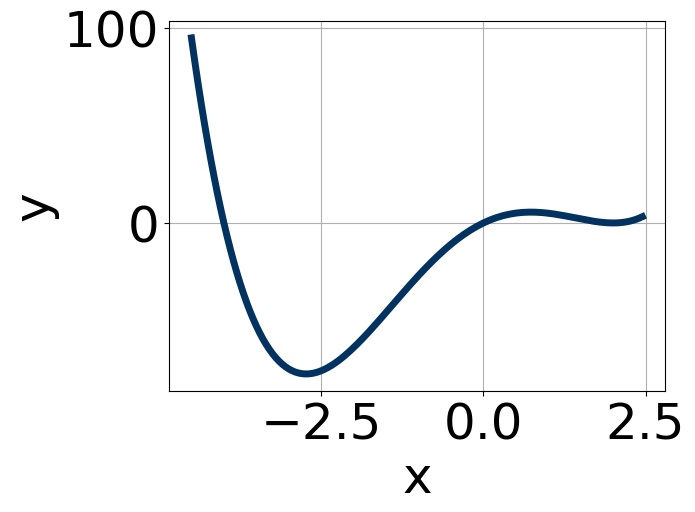
\includegraphics[width=0.5\textwidth]{../Figures/polyGraphToFunctionCopyA.png}
\end{center}


The solution is \( 11x^{9} (x - 2)^{8} (x + 4)^{7} \), which is option D.\begin{enumerate}[label=\Alph*.]
\item \( -18x^{9} (x - 2)^{10} (x + 4)^{8} \)

The factor $(x + 4)$ should have an odd power and the leading coefficient should be the opposite sign.
\item \( 19x^{6} (x - 2)^{9} (x + 4)^{9} \)

The factor $2$ should have an even power and the factor $0$ should have an odd power.
\item \( -14x^{9} (x - 2)^{6} (x + 4)^{5} \)

This corresponds to the leading coefficient being the opposite value than it should be.
\item \( 11x^{9} (x - 2)^{8} (x + 4)^{7} \)

* This is the correct option.
\item \( 19x^{6} (x - 2)^{10} (x + 4)^{9} \)

The factor $x$ should have an odd power.
\end{enumerate}

\textbf{General Comment:} General Comments: Draw the x-axis to determine which zeros are touching (and so have even multiplicity) or cross (and have odd multiplicity).
}
\litem{
Describe the end behavior of the polynomial below.
\[ f(x) = -3(x + 2)^{3}(x - 2)^{8}(x + 6)^{5}(x - 6)^{5} \]The solution is the graph below, which is option A.
    \begin{center}
        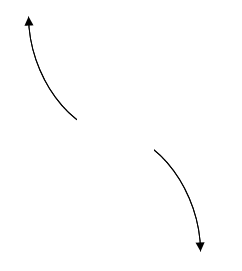
\includegraphics[width=0.3\textwidth]{../Figures/polyEndBehaviorAA.png}
    \end{center}\begin{enumerate}[label=\Alph*.]
\begin{multicols}{2}
\item 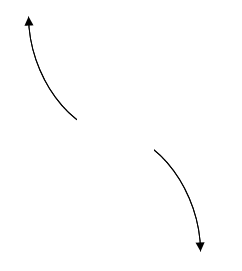
\includegraphics[width = 0.3\textwidth]{../Figures/polyEndBehaviorAA.png}
\item 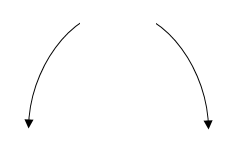
\includegraphics[width = 0.3\textwidth]{../Figures/polyEndBehaviorBA.png}
\item 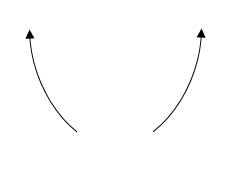
\includegraphics[width = 0.3\textwidth]{../Figures/polyEndBehaviorCA.png}
\item 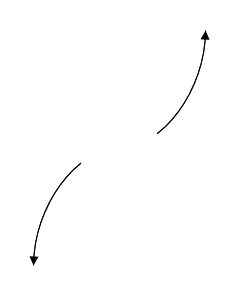
\includegraphics[width = 0.3\textwidth]{../Figures/polyEndBehaviorDA.png}
\end{multicols}\item None of the above.\end{enumerate}
\textbf{General Comment:} Remember that end behavior is determined by the leading coefficient AND whether the \textbf{sum} of the multiplicities is positive or negative.
}
\litem{
Describe the zero behavior of the zero $x = 7$ of the polynomial below.
\[ f(x) = 9(x + 8)^{9}(x - 8)^{7}(x - 7)^{7}(x + 7)^{2} \]The solution is the graph below, which is option A.
    \begin{center}
        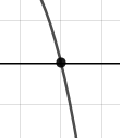
\includegraphics[width=0.3\textwidth]{../Figures/polyZeroBehaviorCopyAA.png}
    \end{center}\begin{enumerate}[label=\Alph*.]
\begin{multicols}{2}
\item 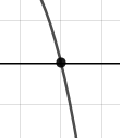
\includegraphics[width = 0.3\textwidth]{../Figures/polyZeroBehaviorCopyAA.png}
\item 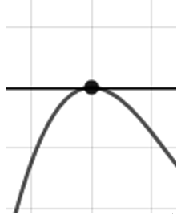
\includegraphics[width = 0.3\textwidth]{../Figures/polyZeroBehaviorCopyBA.png}
\item 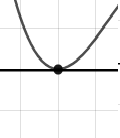
\includegraphics[width = 0.3\textwidth]{../Figures/polyZeroBehaviorCopyCA.png}
\item 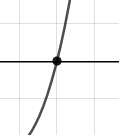
\includegraphics[width = 0.3\textwidth]{../Figures/polyZeroBehaviorCopyDA.png}
\end{multicols}\item None of the above.\end{enumerate}
\textbf{General Comment:} You will need to sketch the entire graph, then zoom in on the zero the question asks about.
}
\litem{
Construct the lowest-degree polynomial given the zeros below. Then, choose the intervals that contain the coefficients of the polynomial in the form $ax^3+bx^2+cx+d$.
\[ \frac{-1}{5}, \frac{-1}{4}, \text{ and } 6 \]The solution is \( 20x^{3} -111 x^{2} -53 x -6 \), which is option E.\begin{enumerate}[label=\Alph*.]
\item \( a \in [16, 21], b \in [107, 116], c \in [-55, -47], \text{ and } d \in [-2, 13] \)

$20x^{3} +111 x^{2} -53 x + 6$, which corresponds to multiplying out $(5x -1)(4x -1)(x + 6)$.
\item \( a \in [16, 21], b \in [-137, -123], c \in [51, 61], \text{ and } d \in [-9, -5] \)

$20x^{3} -129 x^{2} +55 x -6$, which corresponds to multiplying out $(5x -1)(4x -1)(x -6)$.
\item \( a \in [16, 21], b \in [-113, -106], c \in [-55, -47], \text{ and } d \in [-2, 13] \)

$20x^{3} -111 x^{2} -53 x + 6$, which corresponds to multiplying everything correctly except the constant term.
\item \( a \in [16, 21], b \in [-120, -116], c \in [-19, -4], \text{ and } d \in [-2, 13] \)

$20x^{3} -119 x^{2} -7 x + 6$, which corresponds to multiplying out $(5x -1)(4x + 1)(x -6)$.
\item \( a \in [16, 21], b \in [-113, -106], c \in [-55, -47], \text{ and } d \in [-9, -5] \)

* $20x^{3} -111 x^{2} -53 x -6$, which is the correct option.
\end{enumerate}

\textbf{General Comment:} To construct the lowest-degree polynomial, you want to multiply out $(5x + 1)(4x + 1)(x -6)$
}
\litem{
Construct the lowest-degree polynomial given the zeros below. Then, choose the intervals that contain the coefficients of the polynomial in the form $x^3+bx^2+cx+d$.
\[ -5 + 4 i \text{ and } -2 \]The solution is \( x^{3} +12 x^{2} +61 x + 82 \), which is option D.\begin{enumerate}[label=\Alph*.]
\item \( b \in [-14, -10], c \in [53, 67], \text{ and } d \in [-88, -77] \)

$x^{3} -12 x^{2} +61 x -82$, which corresponds to multiplying out $(x-(-5 + 4 i))(x-(-5 - 4 i))(x -2)$.
\item \( b \in [1, 6], c \in [-5, -1], \text{ and } d \in [-8, 0] \)

$x^{3} + x^{2} -2 x -8$, which corresponds to multiplying out $(x -4)(x + 2)$.
\item \( b \in [1, 6], c \in [7, 8], \text{ and } d \in [9, 17] \)

$x^{3} + x^{2} +7 x + 10$, which corresponds to multiplying out $(x + 5)(x + 2)$.
\item \( b \in [9, 25], c \in [53, 67], \text{ and } d \in [82, 90] \)

* $x^{3} +12 x^{2} +61 x + 82$, which is the correct option.
\item \( \text{None of the above.} \)

This corresponds to making an unanticipated error or not understanding how to use nonreal complex numbers to create the lowest-degree polynomial. If you chose this and are not sure what you did wrong, please contact the coordinator for help.
\end{enumerate}

\textbf{General Comment:} Remember that the conjugate of $a+bi$ is $a-bi$. Since these zeros always come in pairs, we need to multiply out $(x-(-5 + 4 i))(x-(-5 - 4 i))(x-(-2))$.
}
\litem{
Construct the lowest-degree polynomial given the zeros below. Then, choose the intervals that contain the coefficients of the polynomial in the form $ax^3+bx^2+cx+d$.
\[ \frac{-5}{4}, \frac{-3}{4}, \text{ and } -5 \]The solution is \( 16x^{3} +112 x^{2} +175 x + 75 \), which is option E.\begin{enumerate}[label=\Alph*.]
\item \( a \in [12, 18], b \in [44, 51], c \in [-145, -143], \text{ and } d \in [73, 83] \)

$16x^{3} +48 x^{2} -145 x + 75$, which corresponds to multiplying out $(4x -5)(4x -3)(x + 5)$.
\item \( a \in [12, 18], b \in [104, 114], c \in [171, 181], \text{ and } d \in [-76, -74] \)

$16x^{3} +112 x^{2} +175 x -75$, which corresponds to multiplying everything correctly except the constant term.
\item \( a \in [12, 18], b \in [72, 73], c \in [-60, -50], \text{ and } d \in [-76, -74] \)

$16x^{3} +72 x^{2} -55 x -75$, which corresponds to multiplying out $(4x -5)(4x + 3)(x + 5)$.
\item \( a \in [12, 18], b \in [-114, -109], c \in [171, 181], \text{ and } d \in [-76, -74] \)

$16x^{3} -112 x^{2} +175 x -75$, which corresponds to multiplying out $(4x -5)(4x -3)(x -5)$.
\item \( a \in [12, 18], b \in [104, 114], c \in [171, 181], \text{ and } d \in [73, 83] \)

* $16x^{3} +112 x^{2} +175 x + 75$, which is the correct option.
\end{enumerate}

\textbf{General Comment:} To construct the lowest-degree polynomial, you want to multiply out $(4x + 5)(4x + 3)(x + 5)$
}
\litem{
Describe the end behavior of the polynomial below.
\[ f(x) = 4(x + 3)^{4}(x - 3)^{9}(x + 2)^{4}(x - 2)^{6} \]The solution is the graph below, which is option D.
    \begin{center}
        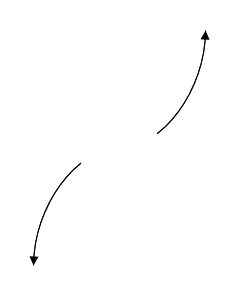
\includegraphics[width=0.3\textwidth]{../Figures/polyEndBehaviorCopyDB.png}
    \end{center}\begin{enumerate}[label=\Alph*.]
\begin{multicols}{2}
\item 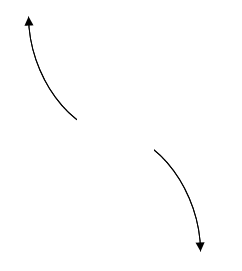
\includegraphics[width = 0.3\textwidth]{../Figures/polyEndBehaviorCopyAB.png}
\item 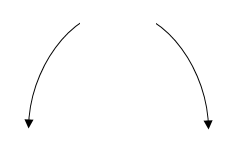
\includegraphics[width = 0.3\textwidth]{../Figures/polyEndBehaviorCopyBB.png}
\item 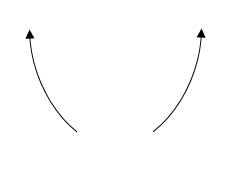
\includegraphics[width = 0.3\textwidth]{../Figures/polyEndBehaviorCopyCB.png}
\item 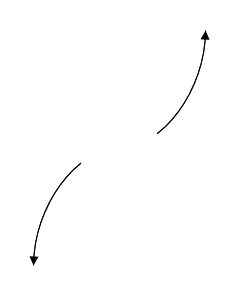
\includegraphics[width = 0.3\textwidth]{../Figures/polyEndBehaviorCopyDB.png}
\end{multicols}\item None of the above.\end{enumerate}
\textbf{General Comment:} Remember that end behavior is determined by the leading coefficient AND whether the \textbf{sum} of the multiplicities is positive or negative.
}
\litem{
Describe the zero behavior of the zero $x = -8$ of the polynomial below.
\[ f(x) = -3(x + 9)^{6}(x - 9)^{5}(x + 8)^{14}(x - 8)^{9} \]The solution is the graph below, which is option B.
    \begin{center}
        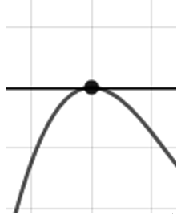
\includegraphics[width=0.3\textwidth]{../Figures/polyZeroBehaviorBB.png}
    \end{center}\begin{enumerate}[label=\Alph*.]
\begin{multicols}{2}
\item 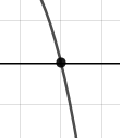
\includegraphics[width = 0.3\textwidth]{../Figures/polyZeroBehaviorAB.png}
\item 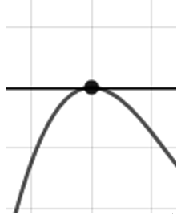
\includegraphics[width = 0.3\textwidth]{../Figures/polyZeroBehaviorBB.png}
\item 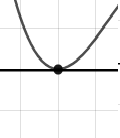
\includegraphics[width = 0.3\textwidth]{../Figures/polyZeroBehaviorCB.png}
\item 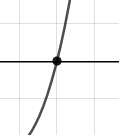
\includegraphics[width = 0.3\textwidth]{../Figures/polyZeroBehaviorDB.png}
\end{multicols}\item None of the above.\end{enumerate}
\textbf{General Comment:} You will need to sketch the entire graph, then zoom in on the zero the question asks about.
}
\litem{
Which of the following equations \textit{could} be of the graph presented below?

\begin{center}
    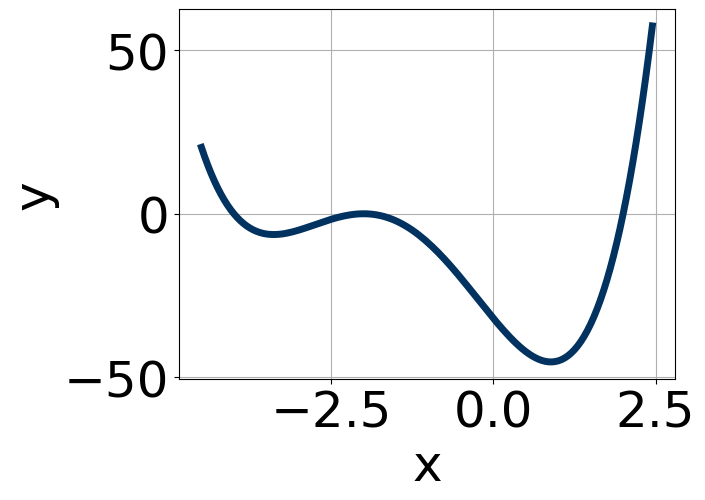
\includegraphics[width=0.5\textwidth]{../Figures/polyGraphToFunctionB.png}
\end{center}


The solution is \( 17(x + 2)^{10} (x - 2)^{7} (x + 4)^{5} \), which is option A.\begin{enumerate}[label=\Alph*.]
\item \( 17(x + 2)^{10} (x - 2)^{7} (x + 4)^{5} \)

* This is the correct option.
\item \( -9(x + 2)^{10} (x - 2)^{9} (x + 4)^{11} \)

This corresponds to the leading coefficient being the opposite value than it should be.
\item \( -18(x + 2)^{10} (x - 2)^{11} (x + 4)^{10} \)

The factor $(x + 4)$ should have an odd power and the leading coefficient should be the opposite sign.
\item \( 8(x + 2)^{7} (x - 2)^{4} (x + 4)^{5} \)

The factor $-2$ should have an even power and the factor $2$ should have an odd power.
\item \( 20(x + 2)^{4} (x - 2)^{4} (x + 4)^{9} \)

The factor $(x - 2)$ should have an odd power.
\end{enumerate}

\textbf{General Comment:} General Comments: Draw the x-axis to determine which zeros are touching (and so have even multiplicity) or cross (and have odd multiplicity).
}
\litem{
Construct the lowest-degree polynomial given the zeros below. Then, choose the intervals that contain the coefficients of the polynomial in the form $x^3+bx^2+cx+d$.
\[ 3 + 2 i \text{ and } 4 \]The solution is \( x^{3} -10 x^{2} +37 x -52 \), which is option C.\begin{enumerate}[label=\Alph*.]
\item \( b \in [1, 8], c \in [-7.52, -6.31], \text{ and } d \in [11, 13] \)

$x^{3} + x^{2} -7 x + 12$, which corresponds to multiplying out $(x -3)(x -4)$.
\item \( b \in [5, 14], c \in [36.76, 37.91], \text{ and } d \in [49, 57] \)

$x^{3} +10 x^{2} +37 x + 52$, which corresponds to multiplying out $(x-(3 + 2 i))(x-(3 - 2 i))(x + 4)$.
\item \( b \in [-15, -7], c \in [36.76, 37.91], \text{ and } d \in [-52, -48] \)

* $x^{3} -10 x^{2} +37 x -52$, which is the correct option.
\item \( b \in [1, 8], c \in [-6.57, -5.83], \text{ and } d \in [6, 9] \)

$x^{3} + x^{2} -6 x + 8$, which corresponds to multiplying out $(x -2)(x -4)$.
\item \( \text{None of the above.} \)

This corresponds to making an unanticipated error or not understanding how to use nonreal complex numbers to create the lowest-degree polynomial. If you chose this and are not sure what you did wrong, please contact the coordinator for help.
\end{enumerate}

\textbf{General Comment:} Remember that the conjugate of $a+bi$ is $a-bi$. Since these zeros always come in pairs, we need to multiply out $(x-(3 + 2 i))(x-(3 - 2 i))(x-(4))$.
}
\litem{
Which of the following equations \textit{could} be of the graph presented below?

\begin{center}
    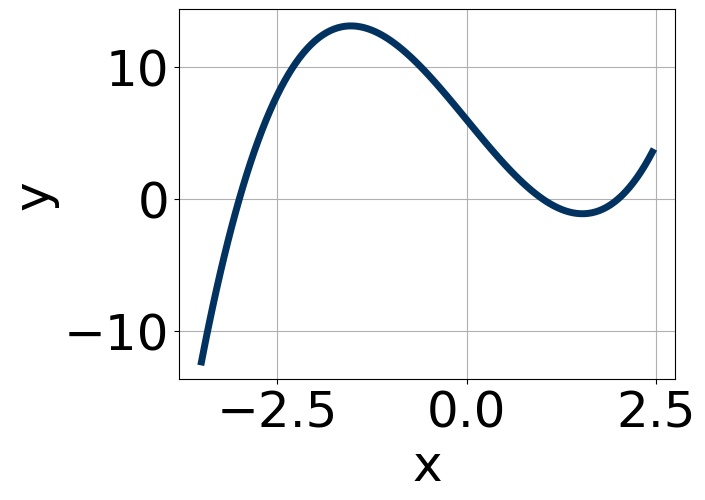
\includegraphics[width=0.5\textwidth]{../Figures/polyGraphToFunctionCopyB.png}
\end{center}


The solution is \( 16(x - 2)^{5} (x + 3)^{5} (x - 1)^{5} \), which is option B.\begin{enumerate}[label=\Alph*.]
\item \( 4(x - 2)^{4} (x + 3)^{6} (x - 1)^{5} \)

The factors $2$ and $-3$ have have been odd power.
\item \( 16(x - 2)^{5} (x + 3)^{5} (x - 1)^{5} \)

* This is the correct option.
\item \( -9(x - 2)^{10} (x + 3)^{9} (x - 1)^{7} \)

The factor $(x - 2)$ should have an odd power and the leading coefficient should be the opposite sign.
\item \( 4(x - 2)^{6} (x + 3)^{7} (x - 1)^{11} \)

The factor $2$ should have been an odd power.
\item \( -10(x - 2)^{11} (x + 3)^{5} (x - 1)^{7} \)

This corresponds to the leading coefficient being the opposite value than it should be.
\end{enumerate}

\textbf{General Comment:} General Comments: Draw the x-axis to determine which zeros are touching (and so have even multiplicity) or cross (and have odd multiplicity).
}
\litem{
Describe the end behavior of the polynomial below.
\[ f(x) = -9(x + 8)^{4}(x - 8)^{5}(x - 6)^{4}(x + 6)^{5} \]The solution is the graph below, which is option B.
    \begin{center}
        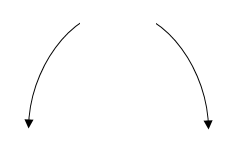
\includegraphics[width=0.3\textwidth]{../Figures/polyEndBehaviorBB.png}
    \end{center}\begin{enumerate}[label=\Alph*.]
\begin{multicols}{2}
\item 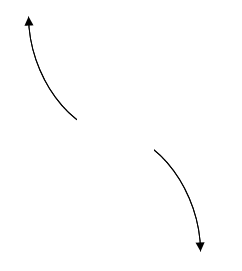
\includegraphics[width = 0.3\textwidth]{../Figures/polyEndBehaviorAB.png}
\item 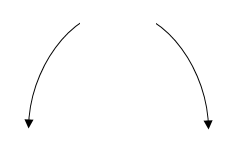
\includegraphics[width = 0.3\textwidth]{../Figures/polyEndBehaviorBB.png}
\item 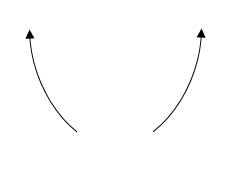
\includegraphics[width = 0.3\textwidth]{../Figures/polyEndBehaviorCB.png}
\item 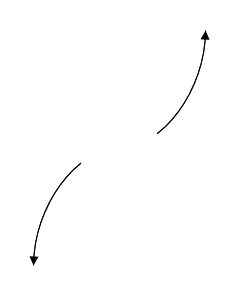
\includegraphics[width = 0.3\textwidth]{../Figures/polyEndBehaviorDB.png}
\end{multicols}\item None of the above.\end{enumerate}
\textbf{General Comment:} Remember that end behavior is determined by the leading coefficient AND whether the \textbf{sum} of the multiplicities is positive or negative.
}
\litem{
Describe the zero behavior of the zero $x = -5$ of the polynomial below.
\[ f(x) = -9(x - 5)^{4}(x + 5)^{7}(x - 9)^{4}(x + 9)^{8} \]The solution is the graph below, which is option A.
    \begin{center}
        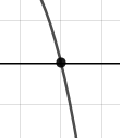
\includegraphics[width=0.3\textwidth]{../Figures/polyZeroBehaviorCopyAB.png}
    \end{center}\begin{enumerate}[label=\Alph*.]
\begin{multicols}{2}
\item 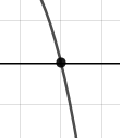
\includegraphics[width = 0.3\textwidth]{../Figures/polyZeroBehaviorCopyAB.png}
\item 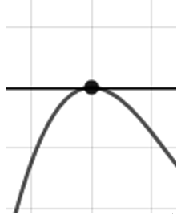
\includegraphics[width = 0.3\textwidth]{../Figures/polyZeroBehaviorCopyBB.png}
\item 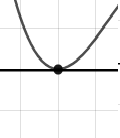
\includegraphics[width = 0.3\textwidth]{../Figures/polyZeroBehaviorCopyCB.png}
\item 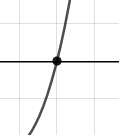
\includegraphics[width = 0.3\textwidth]{../Figures/polyZeroBehaviorCopyDB.png}
\end{multicols}\item None of the above.\end{enumerate}
\textbf{General Comment:} You will need to sketch the entire graph, then zoom in on the zero the question asks about.
}
\litem{
Construct the lowest-degree polynomial given the zeros below. Then, choose the intervals that contain the coefficients of the polynomial in the form $ax^3+bx^2+cx+d$.
\[ 1, \frac{-3}{4}, \text{ and } \frac{6}{5} \]The solution is \( 20x^{3} -29 x^{2} -9 x + 18 \), which is option A.\begin{enumerate}[label=\Alph*.]
\item \( a \in [20, 21], b \in [-35, -25], c \in [-9, 1], \text{ and } d \in [15, 24] \)

* $20x^{3} -29 x^{2} -9 x + 18$, which is the correct option.
\item \( a \in [20, 21], b \in [-22, -14], c \in [-21, -16], \text{ and } d \in [15, 24] \)

$20x^{3} -19 x^{2} -21 x + 18$, which corresponds to multiplying out $(x + 1)(4x -3)(5x -6)$.
\item \( a \in [20, 21], b \in [27, 36], c \in [-9, 1], \text{ and } d \in [-26, -17] \)

$20x^{3} +29 x^{2} -9 x -18$, which corresponds to multiplying out $(x + 1)(4x -3)(5x + 6)$.
\item \( a \in [20, 21], b \in [-35, -25], c \in [-9, 1], \text{ and } d \in [-26, -17] \)

$20x^{3} -29 x^{2} -9 x -18$, which corresponds to multiplying everything correctly except the constant term.
\item \( a \in [20, 21], b \in [10, 12], c \in [-33, -25], \text{ and } d \in [-26, -17] \)

$20x^{3} +11 x^{2} -27 x -18$, which corresponds to multiplying out $(x + 1)(4x + 3)(5x -6)$.
\end{enumerate}

\textbf{General Comment:} To construct the lowest-degree polynomial, you want to multiply out $(x -1)(4x + 3)(5x -6)$
}
\litem{
Construct the lowest-degree polynomial given the zeros below. Then, choose the intervals that contain the coefficients of the polynomial in the form $x^3+bx^2+cx+d$.
\[ 3 + 4 i \text{ and } 4 \]The solution is \( x^{3} -10 x^{2} +49 x -100 \), which is option D.\begin{enumerate}[label=\Alph*.]
\item \( b \in [-5, 7], c \in [-7.9, -4.2], \text{ and } d \in [11, 13] \)

$x^{3} + x^{2} -7 x + 12$, which corresponds to multiplying out $(x -3)(x -4)$.
\item \( b \in [-5, 7], c \in [-8.4, -7.9], \text{ and } d \in [13, 18] \)

$x^{3} + x^{2} -8 x + 16$, which corresponds to multiplying out $(x -4)(x -4)$.
\item \( b \in [7, 19], c \in [48.6, 51.5], \text{ and } d \in [98, 101] \)

$x^{3} +10 x^{2} +49 x + 100$, which corresponds to multiplying out $(x-(3 + 4 i))(x-(3 - 4 i))(x + 4)$.
\item \( b \in [-10, -4], c \in [48.6, 51.5], \text{ and } d \in [-102, -94] \)

* $x^{3} -10 x^{2} +49 x -100$, which is the correct option.
\item \( \text{None of the above.} \)

This corresponds to making an unanticipated error or not understanding how to use nonreal complex numbers to create the lowest-degree polynomial. If you chose this and are not sure what you did wrong, please contact the coordinator for help.
\end{enumerate}

\textbf{General Comment:} Remember that the conjugate of $a+bi$ is $a-bi$. Since these zeros always come in pairs, we need to multiply out $(x-(3 + 4 i))(x-(3 - 4 i))(x-(4))$.
}
\litem{
Construct the lowest-degree polynomial given the zeros below. Then, choose the intervals that contain the coefficients of the polynomial in the form $ax^3+bx^2+cx+d$.
\[ \frac{3}{4}, \frac{5}{2}, \text{ and } -4 \]The solution is \( 8x^{3} +6 x^{2} -89 x + 60 \), which is option C.\begin{enumerate}[label=\Alph*.]
\item \( a \in [5, 9], b \in [16, 29], c \in [-71, -68], \text{ and } d \in [-63, -58] \)

$8x^{3} +18 x^{2} -71 x -60$, which corresponds to multiplying out $(4x + 3)(2x -5)(x + 4)$.
\item \( a \in [5, 9], b \in [-13, -5], c \in [-95, -76], \text{ and } d \in [-63, -58] \)

$8x^{3} -6 x^{2} -89 x -60$, which corresponds to multiplying out $(4x + 3)(2x + 5)(x -4)$.
\item \( a \in [5, 9], b \in [2, 9], c \in [-95, -76], \text{ and } d \in [55, 66] \)

* $8x^{3} +6 x^{2} -89 x + 60$, which is the correct option.
\item \( a \in [5, 9], b \in [2, 9], c \in [-95, -76], \text{ and } d \in [-63, -58] \)

$8x^{3} +6 x^{2} -89 x -60$, which corresponds to multiplying everything correctly except the constant term.
\item \( a \in [5, 9], b \in [57, 64], c \in [115, 125], \text{ and } d \in [55, 66] \)

$8x^{3} +58 x^{2} +119 x + 60$, which corresponds to multiplying out $(4x + 3)(2x + 5)(x + 4)$.
\end{enumerate}

\textbf{General Comment:} To construct the lowest-degree polynomial, you want to multiply out $(4x -3)(2x -5)(x + 4)$
}
\litem{
Describe the end behavior of the polynomial below.
\[ f(x) = 7(x + 5)^{4}(x - 5)^{7}(x - 9)^{3}(x + 9)^{3} \]The solution is the graph below, which is option D.
    \begin{center}
        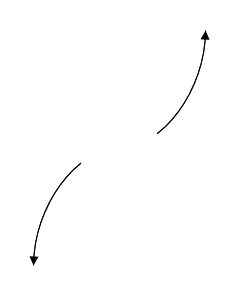
\includegraphics[width=0.3\textwidth]{../Figures/polyEndBehaviorCopyDC.png}
    \end{center}\begin{enumerate}[label=\Alph*.]
\begin{multicols}{2}
\item 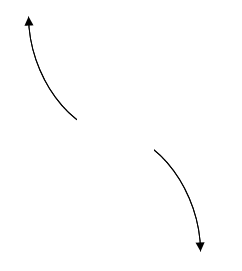
\includegraphics[width = 0.3\textwidth]{../Figures/polyEndBehaviorCopyAC.png}
\item 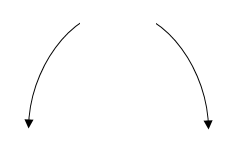
\includegraphics[width = 0.3\textwidth]{../Figures/polyEndBehaviorCopyBC.png}
\item 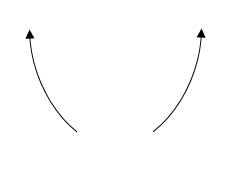
\includegraphics[width = 0.3\textwidth]{../Figures/polyEndBehaviorCopyCC.png}
\item 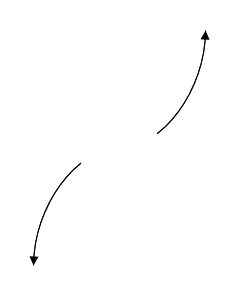
\includegraphics[width = 0.3\textwidth]{../Figures/polyEndBehaviorCopyDC.png}
\end{multicols}\item None of the above.\end{enumerate}
\textbf{General Comment:} Remember that end behavior is determined by the leading coefficient AND whether the \textbf{sum} of the multiplicities is positive or negative.
}
\litem{
Describe the zero behavior of the zero $x = -5$ of the polynomial below.
\[ f(x) = 3(x - 3)^{9}(x + 3)^{7}(x + 5)^{4}(x - 5)^{3} \]The solution is the graph below, which is option B.
    \begin{center}
        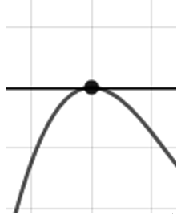
\includegraphics[width=0.3\textwidth]{../Figures/polyZeroBehaviorBC.png}
    \end{center}\begin{enumerate}[label=\Alph*.]
\begin{multicols}{2}
\item \includegraphics[width = 0.3\textwidth]{../Figures/polyZeroBehaviorAC.png}
\item \includegraphics[width = 0.3\textwidth]{../Figures/polyZeroBehaviorBC.png}
\item \includegraphics[width = 0.3\textwidth]{../Figures/polyZeroBehaviorCC.png}
\item \includegraphics[width = 0.3\textwidth]{../Figures/polyZeroBehaviorDC.png}
\end{multicols}\item None of the above.\end{enumerate}
\textbf{General Comment:} You will need to sketch the entire graph, then zoom in on the zero the question asks about.
}
\litem{
Which of the following equations \textit{could} be of the graph presented below?

\begin{center}
    \includegraphics[width=0.5\textwidth]{../Figures/polyGraphToFunctionC.png}
\end{center}


The solution is \( 7(x - 1)^{6} (x - 2)^{11} (x - 3)^{7} \), which is option D.\begin{enumerate}[label=\Alph*.]
\item \( 9(x - 1)^{10} (x - 2)^{8} (x - 3)^{5} \)

The factor $(x - 2)$ should have an odd power.
\item \( 19(x - 1)^{7} (x - 2)^{10} (x - 3)^{5} \)

The factor $1$ should have an even power and the factor $2$ should have an odd power.
\item \( -11(x - 1)^{4} (x - 2)^{11} (x - 3)^{4} \)

The factor $(x - 3)$ should have an odd power and the leading coefficient should be the opposite sign.
\item \( 7(x - 1)^{6} (x - 2)^{11} (x - 3)^{7} \)

* This is the correct option.
\item \( -6(x - 1)^{10} (x - 2)^{11} (x - 3)^{5} \)

This corresponds to the leading coefficient being the opposite value than it should be.
\end{enumerate}

\textbf{General Comment:} General Comments: Draw the x-axis to determine which zeros are touching (and so have even multiplicity) or cross (and have odd multiplicity).
}
\litem{
Construct the lowest-degree polynomial given the zeros below. Then, choose the intervals that contain the coefficients of the polynomial in the form $x^3+bx^2+cx+d$.
\[ 5 + 2 i \text{ and } 4 \]The solution is \( x^{3} -14 x^{2} +69 x -116 \), which is option D.\begin{enumerate}[label=\Alph*.]
\item \( b \in [13, 15], c \in [64, 73], \text{ and } d \in [114, 122] \)

$x^{3} +14 x^{2} +69 x + 116$, which corresponds to multiplying out $(x-(5 + 2 i))(x-(5 - 2 i))(x + 4)$.
\item \( b \in [-4, 5], c \in [-19, -7], \text{ and } d \in [17, 23] \)

$x^{3} + x^{2} -9 x + 20$, which corresponds to multiplying out $(x -5)(x -4)$.
\item \( b \in [-4, 5], c \in [-8, -3], \text{ and } d \in [8, 14] \)

$x^{3} + x^{2} -6 x + 8$, which corresponds to multiplying out $(x -2)(x -4)$.
\item \( b \in [-16, -13], c \in [64, 73], \text{ and } d \in [-125, -112] \)

* $x^{3} -14 x^{2} +69 x -116$, which is the correct option.
\item \( \text{None of the above.} \)

This corresponds to making an unanticipated error or not understanding how to use nonreal complex numbers to create the lowest-degree polynomial. If you chose this and are not sure what you did wrong, please contact the coordinator for help.
\end{enumerate}

\textbf{General Comment:} Remember that the conjugate of $a+bi$ is $a-bi$. Since these zeros always come in pairs, we need to multiply out $(x-(5 + 2 i))(x-(5 - 2 i))(x-(4))$.
}
\litem{
Which of the following equations \textit{could} be of the graph presented below?

\begin{center}
    \includegraphics[width=0.5\textwidth]{../Figures/polyGraphToFunctionCopyC.png}
\end{center}


The solution is \( 2x^{9} (x + 1)^{8} (x + 2)^{10} \), which is option E.\begin{enumerate}[label=\Alph*.]
\item \( 19x^{5} (x + 1)^{6} (x + 2)^{7} \)

The factor $(x + 2)$ should have an even power.
\item \( -14x^{7} (x + 1)^{10} (x + 2)^{4} \)

This corresponds to the leading coefficient being the opposite value than it should be.
\item \( 14x^{6} (x + 1)^{10} (x + 2)^{9} \)

The factor $(x + 2)$ should have an even power and the factor $x$ should have an odd power.
\item \( -11x^{4} (x + 1)^{10} (x + 2)^{4} \)

The factor $x$ should have an odd power and the leading coefficient should be the opposite sign.
\item \( 2x^{9} (x + 1)^{8} (x + 2)^{10} \)

* This is the correct option.
\end{enumerate}

\textbf{General Comment:} General Comments: Draw the x-axis to determine which zeros are touching (and so have even multiplicity) or cross (and have odd multiplicity).
}
\litem{
Describe the end behavior of the polynomial below.
\[ f(x) = -4(x - 4)^{3}(x + 4)^{6}(x + 8)^{5}(x - 8)^{5} \]The solution is the graph below, which is option A.
    \begin{center}
        \includegraphics[width=0.3\textwidth]{../Figures/polyEndBehaviorAC.png}
    \end{center}\begin{enumerate}[label=\Alph*.]
\begin{multicols}{2}
\item \includegraphics[width = 0.3\textwidth]{../Figures/polyEndBehaviorAC.png}
\item \includegraphics[width = 0.3\textwidth]{../Figures/polyEndBehaviorBC.png}
\item \includegraphics[width = 0.3\textwidth]{../Figures/polyEndBehaviorCC.png}
\item \includegraphics[width = 0.3\textwidth]{../Figures/polyEndBehaviorDC.png}
\end{multicols}\item None of the above.\end{enumerate}
\textbf{General Comment:} Remember that end behavior is determined by the leading coefficient AND whether the \textbf{sum} of the multiplicities is positive or negative.
}
\litem{
Describe the zero behavior of the zero $x = 9$ of the polynomial below.
\[ f(x) = -7(x - 9)^{4}(x + 9)^{7}(x + 2)^{6}(x - 2)^{7} \]The solution is the graph below, which is option B.
    \begin{center}
        \includegraphics[width=0.3\textwidth]{../Figures/polyZeroBehaviorCopyBC.png}
    \end{center}\begin{enumerate}[label=\Alph*.]
\begin{multicols}{2}
\item \includegraphics[width = 0.3\textwidth]{../Figures/polyZeroBehaviorCopyAC.png}
\item \includegraphics[width = 0.3\textwidth]{../Figures/polyZeroBehaviorCopyBC.png}
\item \includegraphics[width = 0.3\textwidth]{../Figures/polyZeroBehaviorCopyCC.png}
\item \includegraphics[width = 0.3\textwidth]{../Figures/polyZeroBehaviorCopyDC.png}
\end{multicols}\item None of the above.\end{enumerate}
\textbf{General Comment:} You will need to sketch the entire graph, then zoom in on the zero the question asks about.
}
\litem{
Construct the lowest-degree polynomial given the zeros below. Then, choose the intervals that contain the coefficients of the polynomial in the form $ax^3+bx^2+cx+d$.
\[ \frac{1}{4}, 4, \text{ and } \frac{3}{5} \]The solution is \( 20x^{3} -97 x^{2} +71 x -12 \), which is option A.\begin{enumerate}[label=\Alph*.]
\item \( a \in [12, 21], b \in [-101, -93], c \in [61, 75], \text{ and } d \in [-15, -8] \)

* $20x^{3} -97 x^{2} +71 x -12$, which is the correct option.
\item \( a \in [12, 21], b \in [-101, -93], c \in [61, 75], \text{ and } d \in [8, 15] \)

$20x^{3} -97 x^{2} +71 x + 12$, which corresponds to multiplying everything correctly except the constant term.
\item \( a \in [12, 21], b \in [-88, -82], c \in [23, 26], \text{ and } d \in [8, 15] \)

$20x^{3} -87 x^{2} +25 x + 12$, which corresponds to multiplying out $(4x + 1)(x -4)(5x -3)$.
\item \( a \in [12, 21], b \in [95, 101], c \in [61, 75], \text{ and } d \in [8, 15] \)

$20x^{3} +97 x^{2} +71 x + 12$, which corresponds to multiplying out $(4x + 1)(x + 4)(5x + 3)$.
\item \( a \in [12, 21], b \in [69, 77], c \in [-36, -28], \text{ and } d \in [-15, -8] \)

$20x^{3} +73 x^{2} -31 x -12$, which corresponds to multiplying out $(4x + 1)(x + 4)(5x -3)$.
\end{enumerate}

\textbf{General Comment:} To construct the lowest-degree polynomial, you want to multiply out $(4x -1)(x -4)(5x -3)$
}
\litem{
Construct the lowest-degree polynomial given the zeros below. Then, choose the intervals that contain the coefficients of the polynomial in the form $x^3+bx^2+cx+d$.
\[ -3 + 2 i \text{ and } 1 \]The solution is \( x^{3} +5 x^{2} +7 x -13 \), which is option B.\begin{enumerate}[label=\Alph*.]
\item \( b \in [-8, -3], c \in [7, 8], \text{ and } d \in [11, 14] \)

$x^{3} -5 x^{2} +7 x + 13$, which corresponds to multiplying out $(x-(-3 + 2 i))(x-(-3 - 2 i))(x + 1)$.
\item \( b \in [2, 8], c \in [7, 8], \text{ and } d \in [-16, -8] \)

* $x^{3} +5 x^{2} +7 x -13$, which is the correct option.
\item \( b \in [1, 2], c \in [0, 4], \text{ and } d \in [-5, -2] \)

$x^{3} + x^{2} +2 x -3$, which corresponds to multiplying out $(x + 3)(x -1)$.
\item \( b \in [1, 2], c \in [-7, 1], \text{ and } d \in [0, 5] \)

$x^{3} + x^{2} -3 x + 2$, which corresponds to multiplying out $(x -2)(x -1)$.
\item \( \text{None of the above.} \)

This corresponds to making an unanticipated error or not understanding how to use nonreal complex numbers to create the lowest-degree polynomial. If you chose this and are not sure what you did wrong, please contact the coordinator for help.
\end{enumerate}

\textbf{General Comment:} Remember that the conjugate of $a+bi$ is $a-bi$. Since these zeros always come in pairs, we need to multiply out $(x-(-3 + 2 i))(x-(-3 - 2 i))(x-(1))$.
}
\litem{
Construct the lowest-degree polynomial given the zeros below. Then, choose the intervals that contain the coefficients of the polynomial in the form $ax^3+bx^2+cx+d$.
\[ 4, \frac{-3}{5}, \text{ and } \frac{3}{4} \]The solution is \( 20x^{3} -83 x^{2} +3 x + 36 \), which is option C.\begin{enumerate}[label=\Alph*.]
\item \( a \in [19, 26], b \in [81, 88], c \in [3, 6], \text{ and } d \in [-37, -33] \)

$20x^{3} +83 x^{2} +3 x -36$, which corresponds to multiplying out $(x + 4)(5x -3)(4x + 3)$.
\item \( a \in [19, 26], b \in [76, 78], c \in [-22, -18], \text{ and } d \in [-37, -33] \)

$20x^{3} +77 x^{2} -21 x -36$, which corresponds to multiplying out $(x + 4)(5x + 3)(4x -3)$.
\item \( a \in [19, 26], b \in [-85, -80], c \in [3, 6], \text{ and } d \in [29, 39] \)

* $20x^{3} -83 x^{2} +3 x + 36$, which is the correct option.
\item \( a \in [19, 26], b \in [46, 63], c \in [-101, -94], \text{ and } d \in [29, 39] \)

$20x^{3} +53 x^{2} -99 x + 36$, which corresponds to multiplying out $(x + 4)(5x -3)(4x -3)$.
\item \( a \in [19, 26], b \in [-85, -80], c \in [3, 6], \text{ and } d \in [-37, -33] \)

$20x^{3} -83 x^{2} +3 x -36$, which corresponds to multiplying everything correctly except the constant term.
\end{enumerate}

\textbf{General Comment:} To construct the lowest-degree polynomial, you want to multiply out $(x -4)(5x + 3)(4x -3)$
}
\end{enumerate}

\end{document}